\chapter{РЕЗУЛЬТАТЫ РАБОТЫ}
В качестве результатов работы была произведен теоретико-множественный и теоретико-информационный анализ сложных систем в области поддержки информационной инфраструктуры. Была разработана проблемно-ориентированная систем управления, принятия решений и оптимизации технических объектов в области обслуживания IT. В данной главе представлена модель разработанной системы, архитектура, реализация и результаты испытаний.
\section{Архитектура системы}
Архитектура системы представляет собой модульную систему. Основными компонентами системы являются:
\begin{enumerate}
	\item TU webservice
	\item CoreService
	\item DataService
	\item Reasoner
	\item ClientAgent
	\item MessageBus
\end{enumerate}
Система может работать в 2-х режимах: режим обучения и режим запроса. Вариант использования для режима обучения представлен на Рисунке \ref{img:train}. Главными действующими лицами является специалист технической поддержки (TSS), в общем случае это Пользователь (User). Данный вариант использования имеет несколько ветвей, которые представлены в Таблице \ref{TrainUseCaseTable}.

\begin{table} [htbp]
  \centering
  \parbox{15cm}{\caption{Описание ветвей в Варианте использования "Режим обучения" }\label{TrainUseCaseTable}}
%  \begin{center}
  \begin{tabular}{| p{7cm} || p{7cm} |}
  \hline
  \hline
Ветвь & Описание \\
  \hline
    \hline
communication:Train	& Обучение посредством коммуникации с системой специалиста технической поддержки \\
  \hline
communication:ProvidesSolution  & В случае коммуникации в режиме обучения специалист технической поддержки должен предоставить не только сам запрос, который будет формализован системой, но также решение данного запроса. Система формализует запрос, формализует решение и создаст между ними связи \\
  \hline
communication:ProvideRequest & Специалист технической поддержки вводит в систему запрос \\
  \hline
communication:MonitorsSolution  & Специалист технической поддержки смотрит как применяется решение, если находится проблема, то решение корректируется в посредством запроса CorrectSystemSolutions \\
  \hline
  \hline
  \end{tabular}
%  \end{center}
\end{table}

\begin{figure} [h] 
  \center
  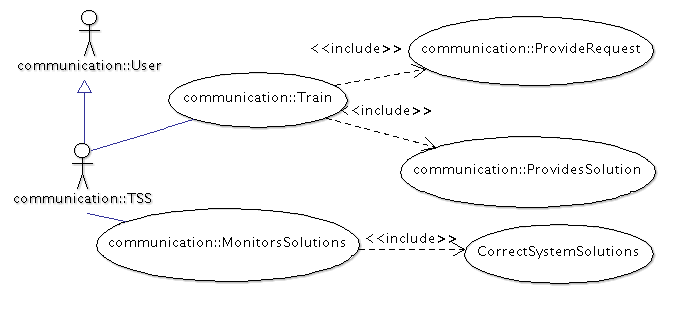
\includegraphics [scale=0.8, angle=90] {UseCaseTrain}
  \caption{Вариант использования. Обучение.} 
  \label{img:train}  
\end{figure}
Второй вариант использования это основной кейс. Главными действующими лицами системы является заказчик (Customer), в общем случае это базовый класс Пользователь (User). Он также имеет несколько ветвей, представленных в Таблице \ref{ProductionUseCase}
\begin{table} [htbp]
  \centering
  \parbox{15cm}{\caption{Описание ветвей в Варианте использования "Основной режим обучения" }\label{ProductionUseCase}}
%  \begin{center}
  \begin{tabular}{| p{7cm} || p{7cm} |}
  \hline
  \hline
Ветвь & Описание \\
  \hline
    \hline
ProvideRequest	& Заказчик вводит запрос в систему на естественном языке. Это может быть либо прямая команда (например, Install Firefox, please), либо описание проблемы  \\
  \hline
communication:ProvideClarificationResponse  &  В случае, если система не может формализовать запрос, либо нашлось множество решений, то система запрашивает пользователя детали
 \\
  \hline
communication:ProvideConfirmationResponse & В случае, когда система нашла решение, она запрашивает пользователя подтверждение о том, что искомое решение решило его проблему
 \\
  \hline
  \hline
  \end{tabular}
%  \end{center}
\end{table}
\clearpage
\subsection{Компоненты системы}
На Рисунке \ref{img:detailed_component_overview} представлена диаграмма компонентов системы. 
\begin{figure} [h] 
  \center
  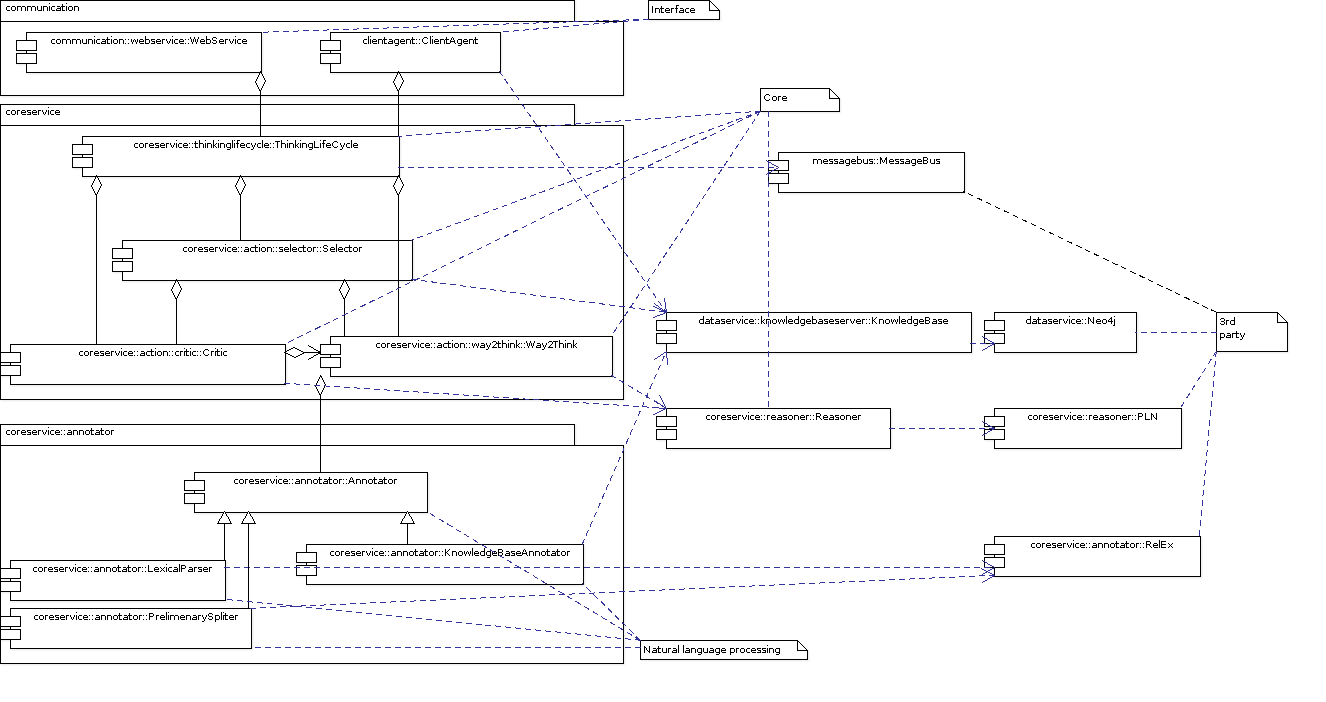
\includegraphics [scale=0.5, angle=90] {detailed_component_overview}
  \caption{Диграма компонентов системы} 
  \label{img:detailed_component_overview}  
\end{figure}
Взаимодействие компонентов системы показано на рисунке \ref{img:main_components_collaboration}.
\begin{figure} [h] 
  \center
  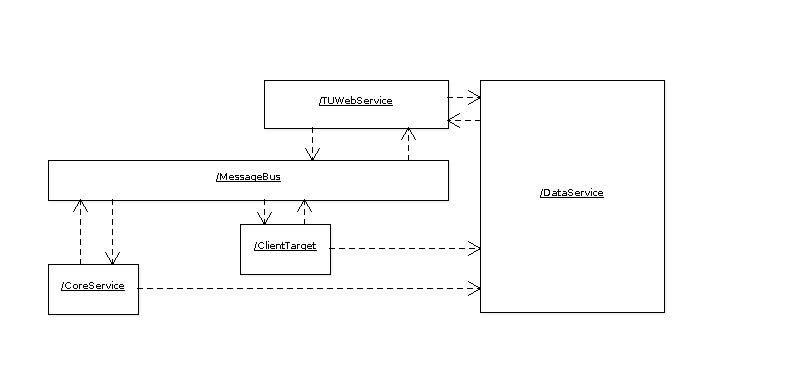
\includegraphics [scale=0.7] {main_components_collaboration}
  \caption{Диграма взаимодействия компонентов} 
  \label{img:main_components_collaboration}  
\end{figure}
Пользователь взаимодействует с системой посредством компонента WebService \ref{WebService}. Взаимодействие происходит по следующей схеме.

\begin{enumerate}
	\item WebService получает запрос пользователя. Сохраняет запрос в Базу Знаний (Базу данных) \ref{Glossary}.
	\item WebService отправляет сообщение типа Request с информацией о запросе в компонент MessageBus (шина).
	\item Один из экземпляров CoreService компонента обрабатывает запрос.
	\item Компонент CoreService обрабатывает запрос и сохраняет результаты в Базу Знаний, затем он отправляет в MessageBus сообщение RequestCompleted и сообщение ActionsToExecute с действиями, которые необходимо исполнить
	\item WebService получает сообщение RequestCompleted c результатами выполнения запроса и уведомляет подписчиков (конечных пользователей)
	\item Компонент ClientAgent получает сообщение ActionsToExecute со списком действий, которые необходимо исполнить на целевых машинах
\end{enumerate}
\clearpage
\subsection{Компонент WebService} \label{WebService}
Данный компонент обрабатывает запросы пользователей. Запрос пользователя представляется объектом Request, который содержит информацию о пользователя, а также ссылку на метод, который будет вызван, когда запрос будет обработан. Вся работа происходит в компоненте CoreService.
На Рисунке \ref{img:web-service-interface} представлен интерфейс компонента.
В Таблице \ref{WebServiceDescription} представлено описание методов.  
\begin{figure} [h] 
  \center
  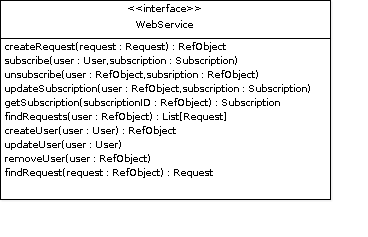
\includegraphics [scale=1.0] {web-service-interface}
  \caption{Интерфейс компонента WebService} 
  \label{img:web-service-interface}  
\end{figure}

\begin{table} [htbp]
   \centering
   \parbox{15cm}{\caption{Описание методов компонента WebService}\label{WebServiceDescription}}
%  \begin{center}
  \begin{tabular}{| p{12cm} ||p{5cm} |}
  \hline
  \hline
Метод & Описание \\
  \hline
  createRequest(request:Request):[RefObject] & Создает запрос от пользователя. В качестве параметра в метод передается SubscriptionID, по которому идет проверка запроса. \\
  
  \hline
  subscribe(user:User,subscription:Subscription)  & Создает подписку для пользователя. \\
  \hline
  unsubscribe(user:RefObject,subscription:RefObject)   & Убирает подписку пользователя. \\
  \hline
  updateSubscription(user:RefObject,subscription:Subscription)   & Обновляет подписку пользователя. \\
  \hline
  getSubscription(subscriptionID:RefObject):List<Request>    & Возвращает подписку. \\
  \hline
  findRequests(user:RefObject)     & Возвращает запросы пользователя. \\
  \hline
  createUser(user:User):RefObject     & Создает пользователя. \\
  \hline
  updateUser(user:User)     & Обновляет информацию о пользователе. \\ 
  \hline
  removeUser(user:RefObject)     & Удаляет информацию о пользователе. \\ 
  \hline
  findRequest(request:RefObject):Request     & Возвращает запрос по ссылке. \\ 
  \hline
  \hline
\end{tabular}
%  \end{center}
\end{table}
Подробное описание классов представлено в \ref{AppendixA}. Основной алгоритм работы компонента:
\begin{enumerate}
	\item Пользователь создает запрос, используя метод WebService.createRequest
	\item Система сохраняет запрос в Базу Знаний и начинает его обработку
	\item Когда изменяется статус запрос request.state система оповещает подписчиков на этот запрос
\end{enumerate}
\clearpage
\subsection{Компонент CoreService.ThinkingLifeCycle} \label{ThinkingLifeCycle}
Это основной компонент системы, ответственный непосредственно за выполнение запросов. Данный компонент управляет потоками, событиями приложения. Он запускает исполнение Критиков (Critic), Селекторов (Selector), Путей мышления (WayToThink), осуществляет обмен данных между компонентами. Компонент построен на фреймворке Akka Concurrency, который позволяет разрабатывать приложения, которые могут работать параллельно \cite{AkkaConcurrency}. \\
В данном компоненте реализовано шесть уровней мышления.
\begin{enumerate}
	\item Instinctive - Инстинктивный уровень
	\item Learned - Уровень обученных реакций
	\item Deliberative - Уровень рассуждений
	\item Reflective - Рефлексивный уровень
	\item Self-Reflective Thinking - Саморефлексивный уровень
	\item Self-Conscious Reflection - Самосознательный уровень
\end{enumerate}

На уровне Instinctive идет обработка сгенерированных по шаблону инцидентов.
Объект, который используется для обработки использует паттерн Akka \cite{AkkaConcurrency}. На рисунке \ref{img:thinking-life-cycle-cd} представлена диаграма классов компонента.  В таблице \ref{TLCCD} представлено описание методов компонента.
\begin{figure} [h] 
  \center
  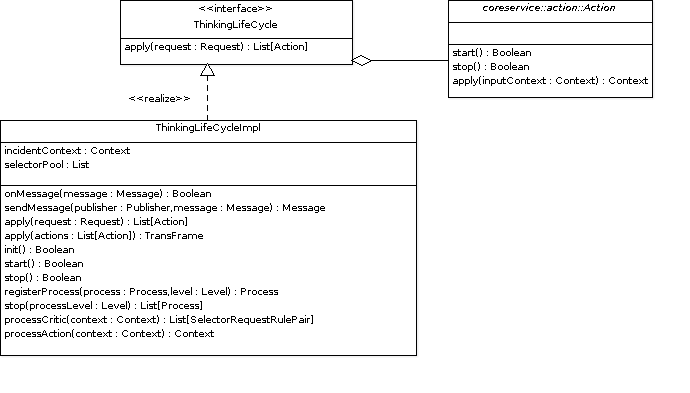
\includegraphics [scale=1.0,angle=90] {thinking-life-cycle-cd}
  \caption{Диаграмма классов ThinkingLifeCycle} 
  \label{img:thinking-life-cycle-cd}  
\end{figure}

\begin{longtable}{|p{7cm}|p{8cm}|}
 \caption[Описание методов класса (компонента) ThinkingLifeCycle]{Описание методов класса (компонента) ThinkingLifeCycle}\label{TLCCD} \\ 
 \hline
 
 \multicolumn{1}{|c|}{\textbf{Метод}} & \multicolumn{1}{c|}{\textbf{Описание}}  \\ \hline 
\endfirsthead
\multicolumn{2}{c}%
{{\bfseries \tablename\ \thetable{} -- продолжение}} \\
\hline \multicolumn{1}{|c|}{\textbf{Метод}} &
\multicolumn{1}{c|}{\textbf{Описание}}  \\ \hline 
\endhead

\hline \multicolumn{2}{|r|}{{Продолжение следует}} \\ \hline
\endfoot

\hline \hline
\endlastfoot
\hline
  onMessage(message : Message) & Данный метод вызывается при получении сообщения от шины. После этого происходит обработка запроса, вычисляется список действий, которые нужно выполнить. После этого запускается исполнение этих действий. На рисунке \ref{img:thinking-life-cycle-on-message-ad} представлена диаграмма действий для этого метода. \\
   \hline
   apply(request : Request) : List[Action] & Данный метод используется для запуска обработки входящего запроса. Для запроса создается контекст, если такой уже не был создан. После этого вызывается следующий компонент системы Selector, который выбирает необходимые ресурсы из базы. На рисунке \ref{img:thinkinglifecycleapplyrequestRequestListAction} представлена диаграмма действий для этого метода.\\
   \hline
   apply(actions : List[Action]) : TransFrame & Данный метод запускает обработку действий. Все действия разделяются на Critic (триггеры действий, которые в итоге должны перейти в WayToThink через Selector) и WayToThink (пути мышления, непосредственно обработчики данных, классы, которые производят изменения данных) На рисунке \ref{img:thinkinglifecycleapplyactionsListActionTransFrame} представлена диаграмма действий для этого метода. \\
   \hline
   processWay2Think(inputContext: Context, outputContext: Context): TransFrame & Данный метод запускает обработку WayToThink \ref{Glossary}. Данный метод создает входной контекст (InputContext), заполняет его параметрами, создает выходной контекст OutputContext. Затем он запускает обработку данных во входном контексте. На рисунке \ref{img:thinkinglifecycleprocessWay2ThinkcontextContext} представлена диаграмма действий для этого метода. \\
    \hline
   processCritic(context: Context):List[SelectorRequestRulePair] & Данный метод запускает обработку Critic \ref{Glossary}. На рисунке \ref{img:thinkinglifecycleactivityprocessCriticcontextContext} представлена диаграмма действий для этого метода. \\
   \hline
   init(): Boolean & Данный метод инициализирует экземпляр класса ThinkingLifeCycle. Во время инициализации происходит Базы Знаний \ref{Glossary}, подключения к Шине данных. На рисунке \ref{img:thinkinglifecycleinitBoolean} представлена диаграмма действий для этого метода. \\
    \hline
   start(): Boolean & Данный метод является оберткой для поддержки Akka Concurrency. Он вызывает метод init. \\
   \hline
   stop(): Boolean & Данный метод является оберткой для поддержки Akka Concurrency. Он останавливает работу экземпляра класса: останавливается сессия к шине данных, останавливается подключение к Базе Знаний.  \\
   \hline
   registerProcess(process : Process,level : Level) : Process & Данный метод регистрирует процесс в пуле. В качестве параметра принимается Level (уровень приоритета процесса). \\
   \hline
   stop(processLevel : Level) : List[Process] & Данный метод регистрирует останавливает процесс. В качестве параметра принимается ссылка на процесс. На рисунке \ref{img:thinkinglifecyclestopprocessLevelLevelListProcess} представлена диаграмма действий для этого метода.  \\

 
 \hline 
\end{longtable}

\begin{figure} [h] 
  \center
  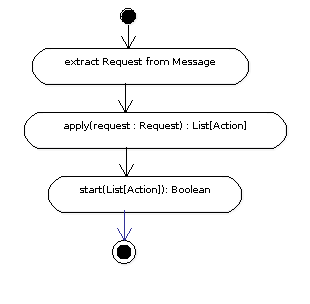
\includegraphics [scale=1.0] {thinking-life-cycle-on-message-ad}
  \caption{Диаграмма действий метода onMessage компонента ThinkingLifeCycle} 
  \label{img:thinking-life-cycle-on-message-ad}  
\end{figure}


\begin{figure} [h] 
  \center
  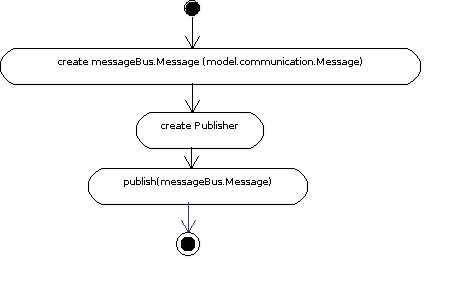
\includegraphics [scale=0.7] {thinking-life-cycle-send-message-publisher-publisher-ad}
  \caption{Диаграмма действий метода sendMessage компонента ThinkingLifeCycle} 
  \label{img:thinking-life-cycle-send-message-publisher-publisher-ad}  
\end{figure}


\begin{figure} [h] 
  \center
  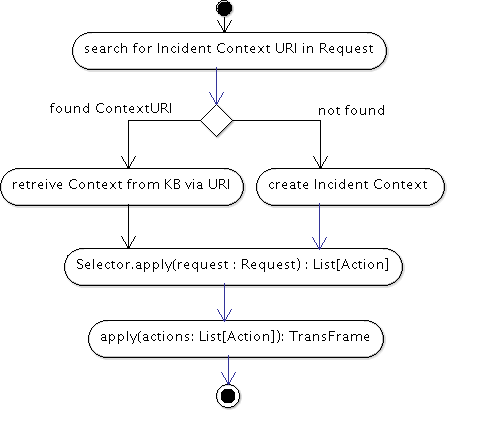
\includegraphics [scale=1.0] {thinkinglifecycleapplyrequestRequestListAction}
  \caption{Диаграмма действий метода apply компонента ThinkingLifeCycle} 
  \label{img:thinkinglifecycleapplyrequestRequestListAction}  
\end{figure}


\begin{figure} [h] 
  \center
  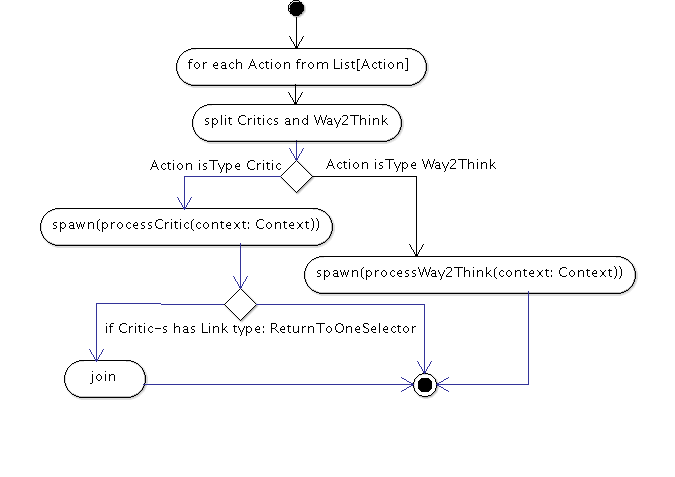
\includegraphics [scale=0.7] {thinkinglifecycleapplyactionsListActionTransFrame}
  \caption{Диаграмма действий метода apply компонента ThinkingLifeCycle} 
  \label{img:thinkinglifecycleapplyactionsListActionTransFrame}  
\end{figure}


\begin{figure} [h] 
  \center
  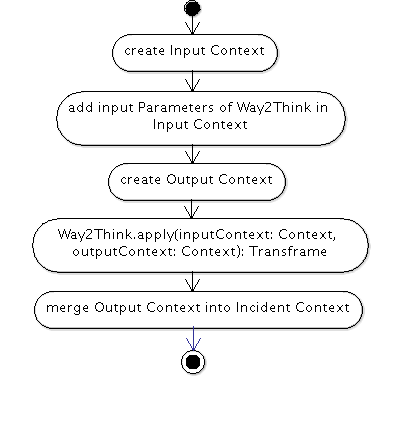
\includegraphics [scale=1.0] {thinkinglifecycleprocessWay2ThinkcontextContext}
  \caption{Диаграмма действий метода processWay2Think компонента ThinkingLifeCycle} 
  \label{img:thinkinglifecycleprocessWay2ThinkcontextContext}  
\end{figure}


\begin{figure} [h] 
  \center
  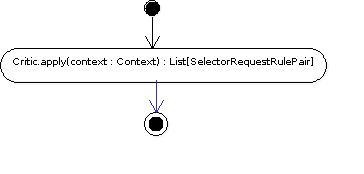
\includegraphics [scale=1.0] {thinkinglifecycleactivityprocessCriticcontextContext}
  \caption{Диаграмма действий метода processCritic компонента ThinkingLifeCycle} 
  \label{img:thinkinglifecycleactivityprocessCriticcontextContext}  
\end{figure}


\begin{figure} [h] 
  \center
  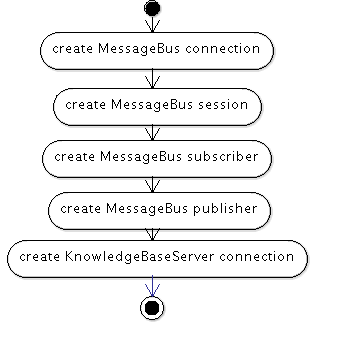
\includegraphics [scale=1.0] {thinkinglifecycleinitBoolean}
  \caption{Диаграмма действий метода init компонента ThinkingLifeCycle} 
  \label{img:thinkinglifecycleinitBoolean}  
\end{figure}

\begin{figure} [h] 
  \center
  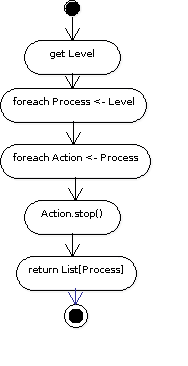
\includegraphics [scale=1.0] {thinkinglifecyclestopprocessLevelLevelListProcess}
  \caption{Диаграмма действий метода stop компонента ThinkingLifeCycle} 
  \label{img:thinkinglifecyclestopprocessLevelLevelListProcess}  
\end{figure}
\clearpage
\subsubsection{Описание работы компонента}
\emph{Запуск и остановка} 
\begin{enumerate}
	\item Когда приложение стартует оно инициализирует ThinkingLifeCycle, который активирует набор критиков, базируясь на текущей цели системы. Например, цель-классифицировать инцидент, активируется набор критиков: разобрать, проверить, найти категорию.
	\item Когда приложение останавливается - оно останавливает все объекты класса и подклассов Actions (Critics, WayToThink), Selectors и ThinkingLifeCycle.
\end{enumerate}
Коммуникация происходит посредством сообщений, отправленных через MessageBus (Шину Данных) \ref{Glossary} JMS \cite{JMS}.
\emph{Взаимодействие компонента с другими компонентами} \\
\begin{enumerate}
	\item Критик возвращает список Селекторов (SelectorRequestRule)
	\begin{enumerate}
	\item ThinkingLifeCycle запускает обработку компонента Selector
	\item Selector возвращает список Action \ref{AppendixB} из базы знаний
	\item ThinkingLifecycle параллельно запускает возвращенные Action
	\begin{enumerate}
	\item Если Action это Critic
	\item ThinkingLifeCycle создает InputContext (входной контекст приложения) и копирует туда все данные из Context (контекста) инцидента
	\item Если Action это Critic с ссылками ReturnToSameSelector ThinkingLifeCycle ждет результаты и отправляет список SelectorRequestRule, возвращенные Critic новому Selector. Иными словами Critic может вернуть новый Selector. В данном случае нам нужно провести операцию Join для всех потоков \cite{JavaConcurrency}. В иных же случаях все Action запускаются в параллельных потоках.
	\end{enumerate} 
	\begin{enumerate}
	\item Если Action это WayToThink
	\item ThinkingLifeCycle создает InputContext (входной контекст приложения) и копирует туда все данные из Context (контекста) возвращенный Selector
	\item TLC \ref{Glossary} запускает WayToThink
	\item TLC сохраняет параметры в OutputContext
	\item TLC сохраняет итоговый результат работы и возвращает его 
	\end{enumerate} 
	\end{enumerate}
\end{enumerate}
\clearpage
%==============================
%==========Selector============
%==============================
\subsection{Компонент CoreService.Selector} \label{Selector}
Selector (Селектор) это компонент, который ответственен за получение списка действий из Базы знаний, согласно входным параметрам.
\textbf{Входной критерий}. TLC запускает Selector c параметрами. 
\textbf{Выходной критерий}. Selector получает список Action: WayToThink или Critic. \\
\begin{figure} [h] 
  \center
  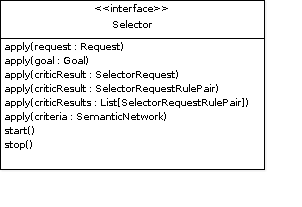
\includegraphics [scale=1.0] {SelectorInterface}
  \caption{Интерфейс компонента Selector} 
  \label{img:SelectorInterface}  
\end{figure}
На Рисунке \ref{img:SelectorInterface} показан интерфейс компонента. В Таблице \ref{SelectorMethodsDescription} приведено описание методов компонента.\\
\begin{longtable}{|p{7cm}|p{8cm}|}
 \caption[Описание методов класса (компонента) Selector]{Описание методов класса (компонента) Selector}\label{SelectorMethodsDescription} \\ 
 \hline
 
 \multicolumn{1}{|c|}{\textbf{Метод}} & \multicolumn{1}{c|}{\textbf{Описание}}  \\ \hline 
\endfirsthead
\multicolumn{2}{c}%
{{\bfseries \tablename\ \thetable{} -- продолжение}} \\
\hline \multicolumn{1}{|c|}{\textbf{Метод}} &
\multicolumn{1}{c|}{\textbf{Описание}}  \\ \hline 
\endhead

\hline \multicolumn{2}{|r|}{{Продолжение следует}} \\ \hline
\endfoot

\hline \hline
\endlastfoot
\hline
  apply(request : Request) : Action & Данный метод на основе запроса пользователя получает из Базы знаний необходимые Critic \ref{Critic}. На рисунке \ref{img:applyrequestRequestActionActivity} представлена диаграмма действий для этого метода. \\
   \hline
   apply(goal: Goal): Данный метод на основе цели системы получает из Базы знаний необходимые Critic \ref{Critic}. На рисунке \ref{img:applygoalGoalActionActivity} представлена диаграмма действий для этого метода.\\
   \hline
   apply(criticResult : ActionProbabilityRule) : Action & Данный метод на основе работы Critic получает из Базы знаний необходимые Action \ref{Action}. На рисунке \ref{img:applycriticResultActionProbabilityRulePairActionActivity} представлена диаграмма действий для этого метода. \\
 \hline 
\end{longtable}

\begin{figure} [h] 
  \center
  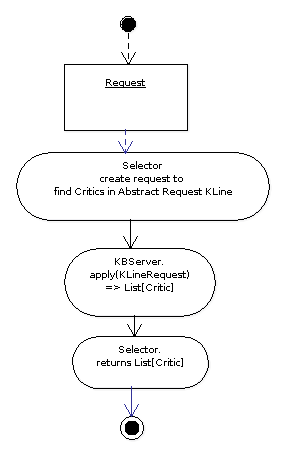
\includegraphics [scale=1.0] {applyrequestRequestActionActivity}
  \caption{Диаграмма действий метода Selector.apply компонента Selector} 
  \label{img:applyrequestRequestActionActivity}  
\end{figure}


\begin{figure} [h] 
  \center
  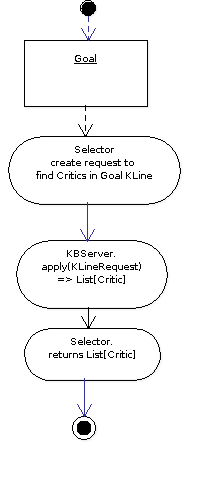
\includegraphics [scale=1.0] {applygoalGoalActionActivity}
  \caption{Диаграмма действий метода Selector.apply компонента Selector} 
  \label{img:applygoalGoalActionActivity}  
\end{figure}

\begin{figure} [h] 
  \center
  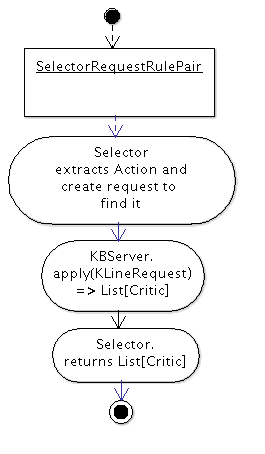
\includegraphics [scale=1.0] {applycriticResultActionProbabilityRulePairActionActivity}
  \caption{Диаграмма действий метода Selector.apply компонента Selector} 
  \label{img:applycriticResultActionProbabilityRulePairActionActivity}  
\end{figure}

\subsubsection{Описание работы компонента}
\textbf{Действия при классификации инцидента}
\begin{enumerate}
	\item TLC \ref{ThinkingLifeCycle} запускает входящие Critic \ref{Critic} параллельно 
	\item Когда Critic возвращает результат работы в виде ActionProbabilityRuleTriple, TLC запускает Selector с этим параметром
	\item Selector запускает GetMostProbableWay2Think, который возвращает наиболее вероятный WayToThink
	\item В некоторых случаях Selector может вернуть менее вероятный вариант, если на Refelective уровне мышления сработал Critic, который посчитал, что данное решение некорректно или же пользователь признал его таким
\end{enumerate}
На Рисунке \ref{img:startRequestProcessingActivity} представлена диаграмма действий выбора наиболее вероятного WayToThink.
\begin{figure} [h] 
  \center
  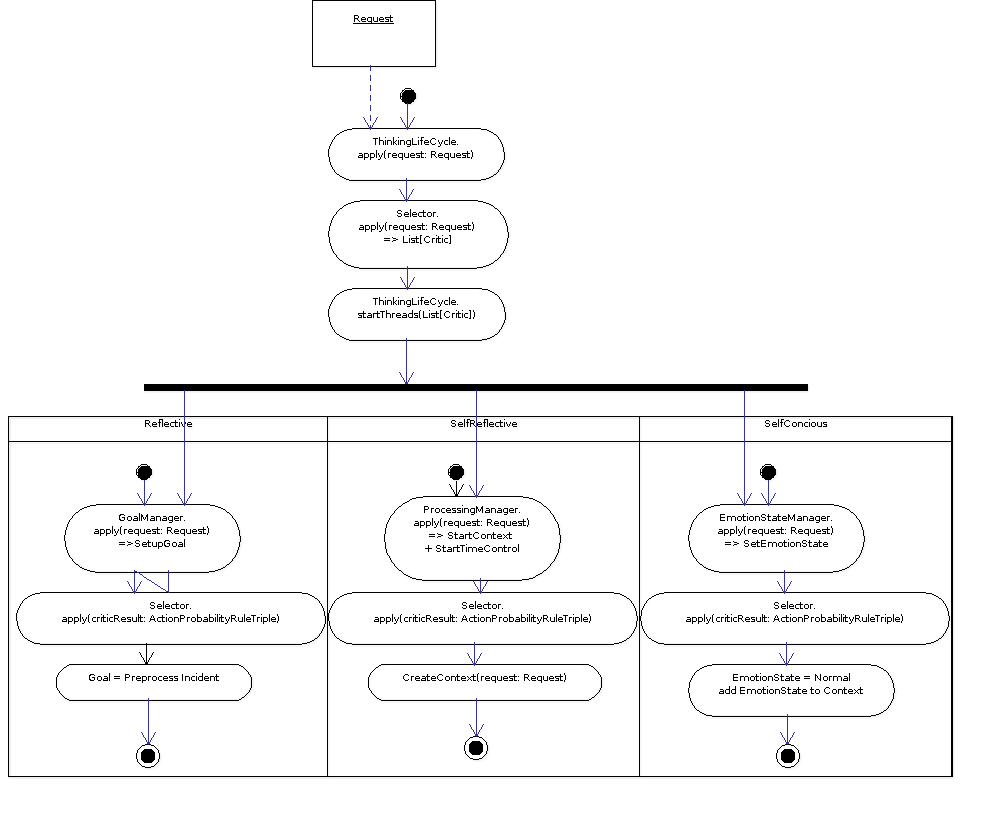
\includegraphics [scale=0.5] {startRequestProcessingActivity}
  \caption{Диаграмма действий выбора WayToThink} 
  \label{img:startRequestProcessingActivity}  
\end{figure}
На Рисунке \ref{img:classifyIncidentActivity} представлена диаграмма действий классификации инцидента. TLC \ref{ThinkingLifeCycle} получает цель Классифицировать инцидент, затем Selector по этой цели возвращает необходимые Critic. Затем TLC запускает обработку Critic в разных потоках (параллельно). В данном случае рассматривает 3 Critic.
\begin{itemize}
	\item DirectInstruction - прямые инструкции, данный Critic возвращает WayToThink Simulate \ref{WayToThink}, который ищет связь между концепциями в запросе и концепциями в Базе Знаний.
	\item ProblemWithDesiredState - проблема с ожидаемым результатом, данный Critic возвращает Simulate+Reformulate WayToThink, которые ищут сопоставление концепциями в Базе Знаний и пытается преобразовать запрос к DirectInstruction запросу (прямым инструкциям).
	\item ProblemWithoutDesiredState - проблема без ожидаемого резульата. Данный Critic возвращает Simulate+Reformulate+InferDesiredState, который пытается преобразовать проблему к ProblemWithDesiredState.
\end{itemize}
Затем TLC собирает результаты выполнения всех Critic и запускает их по новой, пока не будет достигнута изначальная цель.\\
\begin{figure} [h] 
  \center
  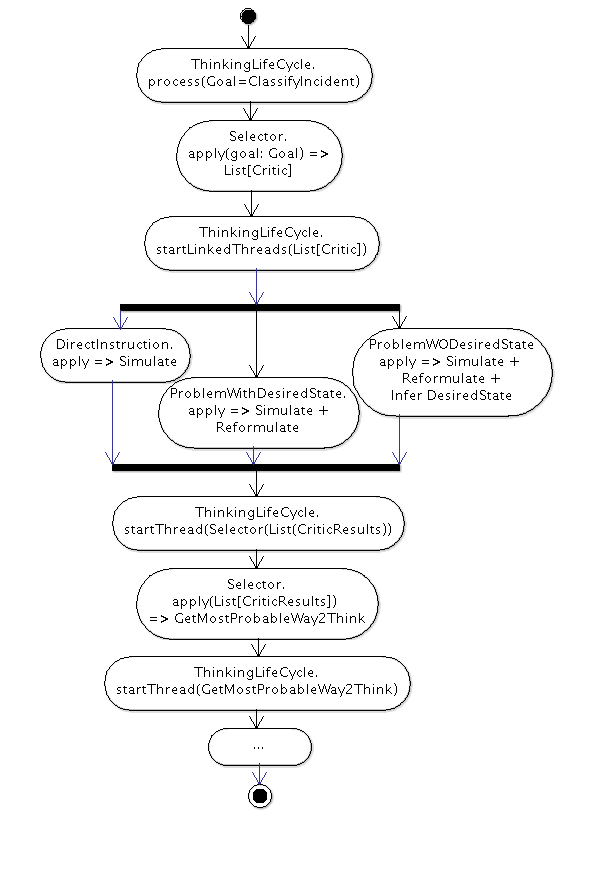
\includegraphics [scale=0.6] {classifyIncidentActivity}
  \caption{Диаграмма действий классификации инцидента} 
  \label{img:classifyIncidentActivity}  
\end{figure}
\clearpage
%============================================
%===============Critic=======================
%============================================
\subsection{Компонент CoreService.Critics} \label{Critic}
Critic является основным компонентом для анализа в триплете Critic->Selector->WayToTHink. Critic используется для классификации входной информации, рефлексии, само-анализа и т.д. и служит определенным вероятностным триггером.\\
\textbf{Входной критерий}\\
TLC \ref{ThinkingLifeCycle} запускает Critic согласно Goal \ref{AppendixC} (Цель) или Request. \\
\textbf{Выходной критерий}\\
Critic генерирует SelectorRequest \ref{Selector}. 
На входе Critic принимает: 
\begin{itemize}
	\item Загруженные из базы правила для работы Critic (CriticRules)
	\item DomainModel:SemanticNetwork - доменная модель, представляющая собой семантическую сеть
	\item Описание инцидента, представляющая собой семантическую сеть
\end{itemize}
На выходе Critic предоставляет следующую информацию:
\begin{itemize}
	\item SelectorRequest \ref{Selector} - запрос на выбор Selector из базы знаний
	\item CriticRules - правило, которое сработало для активации. Данное правило является логическим предикатом
\end{itemize}
На Рисунку \ref{img:CriticApply} представлена диаграмма действий Critic. В Таблице \ref{CriticTypesRaw} приведено описание основных классов Critic. В Таблице \ref{CriticMethods} представлено описание методов компонента Critic.
\begin{figure} [h] 
  \center
  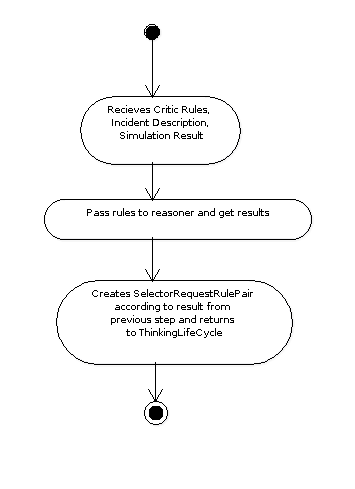
\includegraphics [scale=0.6] {CriticApply}
  \caption{Диаграмма действий компонента Critic} 
  \label{img:CriticApply}  
\end{figure}

\begin{longtable}{|p{7cm}|p{8cm}|}
 \caption[Описание основных классов Critic, используемых в системе]{Описание основных классов Critic, используемых в системе}\label{CriticTypesRaw} \\ 
 \hline
 
 \multicolumn{1}{|c|}{\textbf{Critic}} & \multicolumn{1}{c|}{\textbf{Описание}}  \\ \hline 
\endfirsthead
\multicolumn{2}{c}%
{{\bfseries \tablename\ \thetable{} -- продолжение}} \\
\hline \multicolumn{1}{|c|}{\textbf{Critic}} &
\multicolumn{1}{c|}{\textbf{Описание}}  \\ \hline 
\endhead

\hline \multicolumn{2}{|r|}{{Продолжение следует}} \\ \hline
\endfoot

\hline \hline
\endlastfoot
\hline
   Manager & Простой тип критика, который работает как триггер Goal \ref{AppendixC}, чтобы запустить необходимый WayToThink. \\
   \hline
   Control & контролирующий Critic, который ждет определенного события (срабатывает на определенное событие). Например, заканчивается, отведенное на решение время.\\
   \hline
   Analyser & Анализатор, обрабатывает и выявляет тип инцидента. Например, прямые инструкции, проблема с желаемым состоянием, наиболее вероятное действие. \\
 \hline 
\end{longtable}

\begin{longtable}{|p{7cm}|p{8cm}|}
 \caption[Описание методов класса Critic]{Описание методов компонента Critic}\label{CriticMethods} \\ 
 \hline
 
 \multicolumn{1}{|c|}{\textbf{Метод}} & \multicolumn{1}{c|}{\textbf{Описание}}  \\ \hline 
\endfirsthead
\multicolumn{2}{c}%
{{\bfseries \tablename\ \thetable{} -- продолжение}} \\
\hline \multicolumn{1}{|c|}{\textbf{Метод}} &
\multicolumn{1}{c|}{\textbf{Описание}}  \\ \hline 
\endhead

\hline \multicolumn{2}{|r|}{{Продолжение следует}} \\ \hline
\endfoot

\hline \hline
\endlastfoot
\hline
   exclude():List[CriticLink] & Данный метод возвращает список CriticLink, которые при срабатывание данного Critic будут игнорироваться с определенной вероятностью. После срабатывания Critic, будет посчитана суммарная вероятность активации. После чего система решит, какой Critic был в действительности активирован. \\
   \hline
   include():List[Critic] & Данный метод возвращает список CriticLink, которые при срабатывание данного Critic будут включаться с определенной вероятностью.\\
   \hline
   apply(currentSituation:SemanticNetwork, domainModel:SemanticNetwork): List[SelectorRequestRulePair] & Данный метод запускает Critic, после чего вернется список Selector \ref{Selector} с определенной веротяностью, после чего TLC \ref{ThinkingLifeCycle} их активирует. \\
 \hline 
\end{longtable}
\clearpage
Основные примеры Critic с привязкой к уровням мышления:
\begin{enumerate}
	\item Уровень обученных реакций
	\begin{enumerate}
		\item PreprocessManager - предобработка информации
		\item Классификаторы инцидентов: Прямые инструкции, Проблема с желаемым состоянием, Проблема без желаемого состояния
		\item SolutionCompletenessManager - связывается с пользователем и проверяет устраивает ли его найденное решение
	\end{enumerate}
	\item Уровень рассуждений
	\begin{enumerate}
		\item Выбор наиболее вероятного Selector по Rule. Данный Critic после проверки правил, выбирает из них правило с большей вероятностью
	\end{enumerate}
	\item Рефлексивный уровень
	\begin{enumerate}
		\item Менеджер целей. Установка целей
	\end{enumerate}
	\item Саморефлексивный уровень
	\begin{enumerate}
		\item ProcessingManager - запускает выполнение запроса
		\item TimeControl - контроль времени исполнения запроса
		\item DoNotUnderstandManager - активируется, когда необходимо уточнение пользователя для продолжения работы
	\end{enumerate}
	\item Самосознательный уровень
	\begin{enumerate}
		\item EmotionalStateManager - контроль общего состояния системы
	\end{enumerate} 
\end{enumerate}
\clearpage
%=================================
%===========WayToThink============
%=================================
\subsection{Компонент CoreService.WayToThink} \label{WayToThink}
WayToThink является основным операционным компонентом триплета Critic->Selector->WayToThink. Основными задачами данного компонента являются: обновление, преобразование, сохранение данных и коммуникация с пользователем. \\
\textbf{Входной критерий}\\
Запуска из компонента ThinkingLufeCycle \ref{ThinkingLifeCycle}. Входными данными является InputContext, который содержит параметры WayToThink.\\
\textbf{Выходной критерий}\\
WayToThink завершил работу. На выходе возвращается измененные данные в ходе работе.\\
На Рисунке \ref{img:Way2ThinkInterface} представлен интерфейс компонента. \\
\begin{figure} [h] 
  \center
  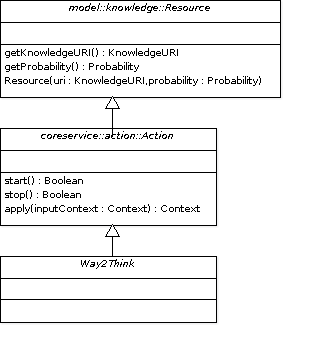
\includegraphics [scale=0.6] {Way2ThinkInterface}
  \caption{Интерфейс компонента WayToThink} 
  \label{img:Way2ThinkInterface}  
\end{figure}
В общем виде компонент описывает последовательность действий. В системе используется два больших класса WaytToThink простой и составной (сложный). Простые WayToThink являются встроенными в систему, остальные являются комбинацией компонентов: Critic \ref{Critic}, Selector \ref{Selector}, WayToThink \ref{WayToThink}. В Таблице \ref{WayToThinkList} приведено описание встроенных в систему WayToThink. В Таблице \ref{WayToThinkMethods} представлено описание методов WayToThink.  \\
\begin{longtable}{|p{7cm}|p{8cm}|}
 \caption[Описание встроенных в систему WayToThink]{Описание встроенныъ в систему WayToThink}\label{WayToThinkList} \\ 
 \hline
 
 \multicolumn{1}{|c|}{\textbf{WayToThink}} & \multicolumn{1}{c|}{\textbf{Описание}}  \\ \hline 
\endfirsthead
\multicolumn{2}{c}%
{{\bfseries \tablename\ \thetable{} -- продолжение}} \\
\hline \multicolumn{1}{|c|}{\textbf{WayToThink}} &
\multicolumn{1}{c|}{\textbf{Описание}}  \\ \hline 
\endhead

\hline \multicolumn{2}{|r|}{{Продолжение следует}} \\ \hline
\endfoot

\hline \hline
\endlastfoot
\hline
   Создать контекст & Данный WayToThink создает объект Context для аккумуляции данных запроса. \\
   \hline
   Установить общий статус системы & Данный WayToThink устанавливает состояние системы в глобальном контексте.\\
   \hline
   Установить цель системы & Данный WayToThink устанавливает цель запроса в текущем контексте  \ref{AppendixC}. \\
    \hline
   Разделить фразу на слова и предложения & Данный WayToThink разбивает фразу на слова и возвращает список слов.\\
    \hline
   Найти связи между входной информацией и базой знаний & Данный WayToThink ищет связь между входной информацией и базой знаний.\\ 
   \hline
   Извлечь связи & Данный WayToThink возвращает список связей из фразы.\\
    \hline
   Сохранить наиболее вероятное решение & Данный WayToThink сохраняет наиболее вероятное решение.\\
    \hline
   Перефразировать (Reformulate) & Данный WayToThink ищет связь между текущим контекстом и известными проблемами, если есть неизвестные концепции, то он пытается их переформулировать при помощи пользотеля.\\
   \hline
   Смоделировать (Simulate) & Данный WayToThink ищет связь между текущим контекстом и проблемами уже сохраненными в базе.\\
   \hline
   Найти решение & Данный WayToThink производит поиск решения, которое прикреплено к проблеме, которая была найдена при помощи моделирования и перефразирования.\\
   \hline
   Остановить работу & Данный WayToThink останавливает работу системы.\\
 \hline 
\end{longtable}

\begin{longtable}{|p{7cm}|p{8cm}|}
 \caption[Описание методов компонента WayToThink]{Описание методов компонента WayToThink}\label{WayToThinkMethods} \\ 
 \hline
 
 \multicolumn{1}{|c|}{\textbf{Метод}} & \multicolumn{1}{c|}{\textbf{Описание}}  \\ \hline 
\endfirsthead
\multicolumn{2}{c}%
{{\bfseries \tablename\ \thetable{} -- продолжение}} \\
\hline \multicolumn{1}{|c|}{\textbf{Метод}} &
\multicolumn{1}{c|}{\textbf{Описание}}  \\ \hline 
\endhead

\hline \multicolumn{2}{|r|}{{Продолжение следует}} \\ \hline
\endfoot

\hline \hline
\endlastfoot
\hline
   start() & Запустить обработку информации. \\
   \hline
   stop() & Остановить обработку, например, если выполнение идет слишком долго.\\
   \hline
   apply(inputContext:Context):Context & Применить WayToThink. Исполнение начнется только после вызова метода start. \\
    \hline
\end{longtable}

WayToThink также используется как Решение (HowTo) \ref{AppendixDHowTo} , то есть описывает последовательность действий, необходимых для решения проблемы. 
\begin{figure} [h] 
  \center
  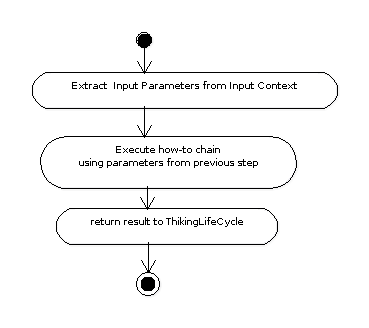
\includegraphics [scale=0.6] {way2thinkHowToActivity}
  \caption{Работа компонента WayToThink в режиме Рецепта решения (HowTo) } 
  \label{img:way2thinkHowToActivity}  
\end{figure}
%===================================
%===========PreliminaryAnnotator====
%===================================
\clearpage
\subsection{Компонент CoreService.PrelimenaryAnnotator} \label{PreliminaryAnnotator}
Данный компонент проводит предварительную подготовку текста: грамматическую и орфографическую коррекцию текста, а также разделение на предложения. На Рисунке \ref{img:PrelimenaryAnnotatorInterface} представлен интерфейс компонента. Компонент также является WayToThink, так как он производит модификацию данных контекста. В Таблице \ref{PrelimenaryAnnotatorMethods} приведено описание методов класса.
\begin{figure} [h] 
  \center
  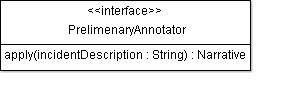
\includegraphics [scale=0.6] {PrelimenaryAnnotatorInterface}
  \caption{Интерфейс компонента PrelimenaryAnnotator} 
  \label{img:PrelimenaryAnnotatorInterface}  
\end{figure}
\begin{longtable}{|p{7cm}|p{8cm}|}
 \caption[Описание методов компонента PrelimenaryAnnotator]{Описание методов компонента PrelimenaryAnnotator}\label{PrelimenaryAnnotatorMethods} \\ 
 \hline
 
 \multicolumn{1}{|c|}{\textbf{Метод}} & \multicolumn{1}{c|}{\textbf{Описание}}  \\ \hline 
\endfirsthead
\multicolumn{2}{c}%
{{\bfseries \tablename\ \thetable{} -- продолжение}} \\
\hline \multicolumn{1}{|c|}{\textbf{Метод}} &
\multicolumn{1}{c|}{\textbf{Описание}}  \\ \hline 
\endhead

\hline \multicolumn{2}{|r|}{{Продолжение следует}} \\ \hline
\endfoot

\hline \hline
\endlastfoot
\hline
   apply(incidentDescription:String):Narrative & Данный метод запускает обработку входного текста и его корректировку. \\
   \hline
  \end{longtable}
\clearpage
%===================================
%===========KnowledgeBaseAnnotator==
%===================================
\subsection{Компонент CoreService.KnowledgeBaseAnnotator} \label{KnowledgeBaseAnnotator}
Данный компонент устанавливает связи между терминами во входной фразе и базой знаний. Данный компонент также является WayToThink \ref{WayToThink}.  \\
\textbf{Входными критериями} является список фраз. \\
\textbf{Выходными критериями} является список ссылок на внутренние термины. \\
\textbf{Описание работы компонента:}
\begin{enumerate}
	\item Получен Термин
	\item Поиск в локальной базе знаний
	\item Если совпадение не найдено идет запрос во внешнюю базу знаний
	\item Внешняя база возвращает список синонимов
	\item Компонент ищет по синонимам во внутренний базе знаний
	\item Если поиск успешен, то создается связь между входящем термином, синонимом и концепцией в базе знаний
\end{enumerate}
Например, входящий запрос содержит термин 'program', База знаний содержит термин 'computer software'. Идет запрос во внешние базы знаний, найдено computer software, program. Будет добавлена аналогия в база знаний program->computer software. 

\clearpage
%===================================
%===========DataService==
%===================================
\subsection{Компонент DataService} \label{data service}
Данный компонент отвечает за хранение данных в системе. База знаний построена на графах. На Рисунке \ref{img:KnowledgeBaseServer} представлен интерфейс компонента. В базе знаний используется два типа объектов Object - объект базы знаний, BusiessObject - объект для Web Service (User, Request). BusinessObject является кортежем для интеграции с внешними системами. У объекта есть ID, который уникально удостоверяет его в рамках системы. В Таблице \ref{DataServiceMethods} приведено описание методов компонента. \\
\begin{figure} [h] 
  \center
  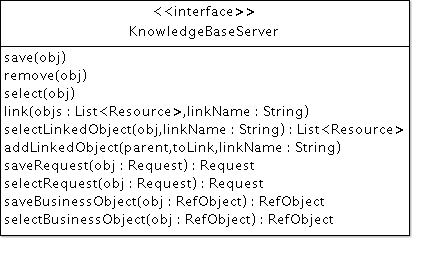
\includegraphics [scale=0.6] {KnowledgeBaseServer}
  \caption{Интерфейс компонента KnowledgeBaseServer} 
  \label{img:KnowledgeBaseServer}  
\end{figure}
\begin{longtable}{|p{7cm}|p{8cm}|}
 \caption[Описание методов компонента DataService]{Описание методов компонента DataService}\label{DataServiceMethods} \\ 
 \hline
 
 \multicolumn{1}{|c|}{\textbf{Метод}} & \multicolumn{1}{c|}{\textbf{Описание}}  \\ \hline 
\endfirsthead
\multicolumn{2}{c}%
{{\bfseries \tablename\ \thetable{} -- продолжение}} \\
\hline \multicolumn{1}{|c|}{\textbf{Метод}} &
\multicolumn{1}{c|}{\textbf{Описание}}  \\ \hline 
\endhead

\hline \multicolumn{2}{|r|}{{Продолжение следует}} \\ \hline
\endfoot

\hline \hline
\endlastfoot
\hline
   save(obj:Resource): Resource  & Данный метод позволяет сохранить ресурс в базу знаний. \\
   \hline
   remove(obj:Resource)  & Данный метод позволяет удалить объект. \\
   \hline
   select(obj:Resource): Resource  & Данный метод позволяет выбрать объект. \\
   \hline
   link(obj:List<Resource>,linkName:String)  & Данный метод позволяет сделать ссылку между 2-мя объектами. \\
   \hline
   selectLinkedObject(obj:Resource, linkName:String): Link<Resource>  & Данный метод позволяет выбрать все объекты, которые имеют связь под названием linkName с объектом obj. \\
   \hline
   addLinkedObject(parent:Resource, toLink:Resource, linkName:String)  & Данный метод позволяет создать ссылку linkName с объектом. \\
   \hline
   saveRequest(obj:Request)  & Данный метод позволяет получить запрос из Базы Знаний. \\
   \hline
   selectRequest(obj:RefObject)  & Данный метод позволяет получить запрос из Базы Знаний. \\
   \hline
   saveBusinessObject(obj:RefObject): RefObject  & Данный метод позволяет сохранить объект в базу. \\
   \hline
   selectBusinessObject(obj:RefObject): RefObject  & Данный метод позволяет полуить объект из Базы Знаний. \\
   \hline
  \end{longtable}
%=================================
%===========ClientAgent===========
%=================================
\subsection{Компонент ClientAgent} \label{client agent}
Данный компонент предназначен для выполнения решений на конечной машине. Данный компонент должен поддерживать обработку (см. Приложение \ref{AppendixDHowTo}). В случае проблем компонент также должен обращаться за помощью к специалисту.
\clearpage

%=================================
%===========Knowledge=============
%=================================
\section{Модель данных системы - TU Knowledge}
Для работы системы была разработана уникальная схема данных - TU Knowledge, которая сочетает в себе OWL и графовую базу данных. Язык OWL, родившейся для структурирования информации Web \cite{OWL} обрел широкое использование во многих схемах данных, так как давал возможность дополнительного расширенного описания взаимосвязи между данными. На Рисунке \ref{img:KnowledgeClass} представлена схема данных TU Knowledge. В Таблице \ref{TUKnowledge} представлено описание схемы TU Knowledge.
\begin{figure} [h] 
  \center
  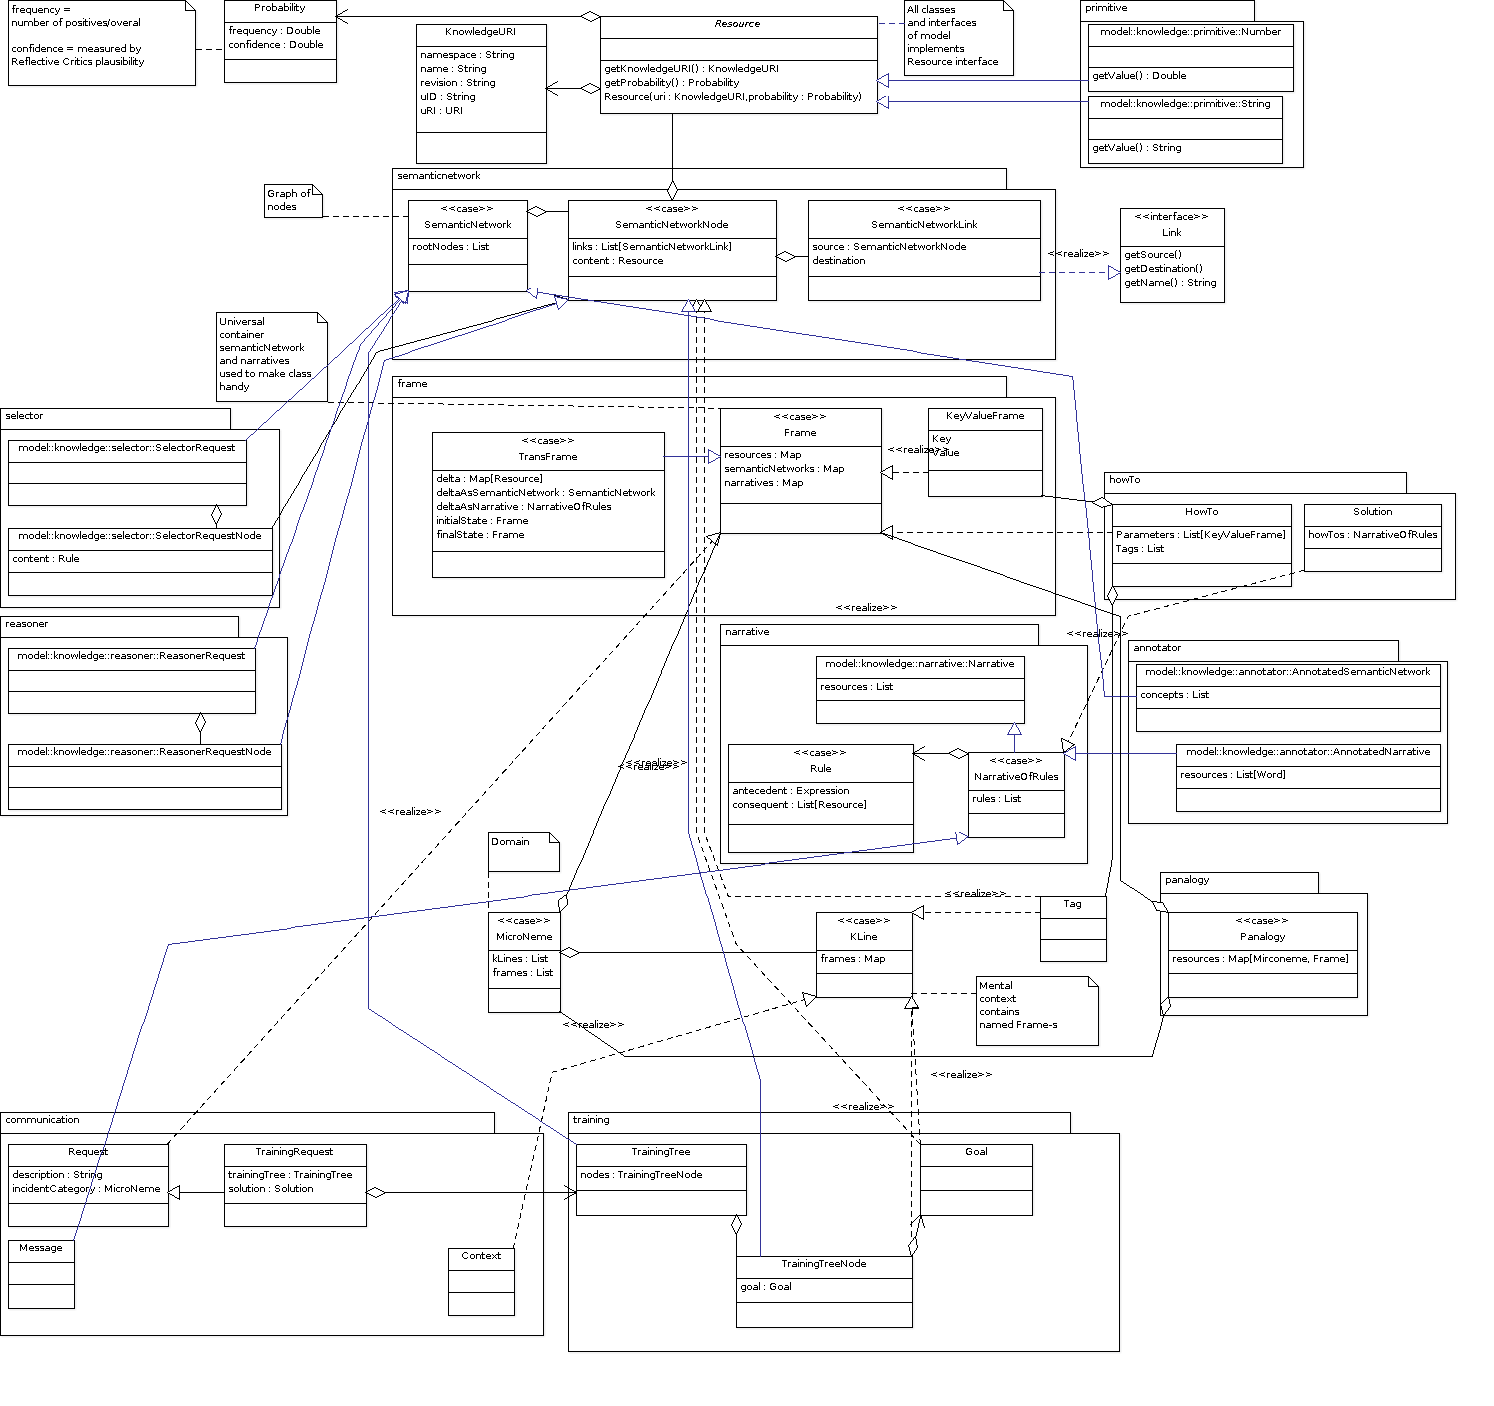
\includegraphics [scale=0.33] {KnowledgeClass}
  \caption{Схема данных TU Knowledge в формате UML} 
  \label{img:KnowledgeClass}  
\end{figure}

\begin{longtable}{|p{5cm}|p{10cm}|}
 \caption[Описание классов TUKnowledge]{Описание классов TUKnowledge}\label{TUKnowledge} \\ 
 \hline
 
 \multicolumn{1}{|c|}{\textbf{Класс}} & \multicolumn{1}{c|}{\textbf{Описание}}  \\ \hline 
\endfirsthead
\multicolumn{2}{c}%
{{\bfseries \tablename\ \thetable{} -- продолжение}} \\
\hline \multicolumn{1}{|c|}{\textbf{Класс}} &
\multicolumn{1}{c|}{\textbf{Описание}}  \\ \hline 
\endhead

\hline \multicolumn{2}{|r|}{{Продолжение следует}} \\ \hline
\endfoot

\hline \hline
\endlastfoot
\hline
   Knowledge  & Базовый класс всех объектов модели. Содержит в себе URI, по которому уникально идентифицируется. Поддерживает версионность. Свойствами данного объекта обладают все объекты системы. Также содержит Probability (Вероятность) и Confidence (Уверенность) поля. Например, когда в результате работу WayToThink получается Knowledge он имеет Confidence 0, так как он только что был сгенерирован, когда его проверит Critic на его состоятельность при помощи определенных в Critic правил, то он поставит ему не 0 Confidence. \\
   \hline
   Narrative  & Список слов исходного запроса. \\
   \hline
   Rule  & Правило. Класс описывающий правила в системы. Например, правило по которому сработает Critic \ref{Critic}.  \\
   \hline
   AnnotatedNarrative  & Слова исходного запроса и их сопоставление на концепции в Базе Знаний \\
   \hline
   SemanticNetwork  & Граф из SemanticNetworkNode и SemanticNetworkLink. \\
   \hline
   SemanticNetworkNode  & Узел графа SemanticNetwork, содержит в себе ссылки на другие узлы, а также ссылку на Knowledge. \\
   \hline
   SemanticNetworkLink  & Ссылка в графе SemanticNetworkLink. \\
   \hline
   Frame  & Коллекция объектов Knowledge, с возможностью проставление специального тега для семантической группировки. \\
   \hline
   TransFrame  & Коллекция Frame, содержащая два состояния одного фрейма: до и после. \\
   \hline
   Goal  & Цель. Приложение \ref{AppendixC}. \\
   \hline
   Tag & Тоже что и цель, но использующиеся для меток. \\
   \hline
   Preliminary annotation  & SemanticNetwork входного запроса. \\
   \hline
   KnowledgeBase annotation  & SemanticNetwork с сопостовлением концепциям Базы Знаний. \\
   \hline
   Domain model  & SemanticNetwork доменной модели. \\
   \hline
   Situation model  & SemanticNetwork, часть DomainModel, созданной для обработки текущего запроса. Приложение \ref{AppendixB}. \\
   \hline
   Incident  & SemanticNetwork входного запроса к систему. \\
   \hline
   K-Line  & Связь между объектами. Например, когда в систему поступает запрос она создает K-Line между Conversation, Narrative. \\
   \hline
   Conversation  & SemanticNetwork, контекст инцидента. \\
   \hline
   InboundRequest  & SemanticNetwork входного запроса. \\
   \hline
   Training Request  & SemanticNetwork входного запроса для обучений. \\
   \hline
   
  \end{longtable}

\clearpage
%=================================
%===========Prototype=============
%=================================
\section{Прототип}
В прототипе были реализованы 4 уровня мышления. Основной рабочий поток приложения описан следующим алгоритмом:
\begin{enumerate}
	\item Поступает запрос от пользователя \\
	User had received wrong application.
User has ordered Wordfinder Business Economical.
However she received wrong version, she received Wordfinder Tehcnical instead of Business Economical. Please assist.
	\item GoalManger устанавливает цель системы HelpUser
	\item Активируется набор Critic, привязанный к данной цели
	\item PreliminaryAnnorator разбирает фразу
	\item KnowledgeBaseAnnotator создает семантическую сеть и ссылки на нее
	\item Critic на Рефликсивном уровне запускает WayToThink ProblemSolving с целью: ResolveIncident
	\item Critic на Рефликсивном уровне выбирает WayToThink KnowingHow
	\begin{enumerate}
	\item Запускаются параллельно все Critic, которые привязаны к IncidentClassification Critic, который привязан к ResolveIncident цели, в данном случае это DirectInstruction, ProblemWithDesiredState, ProblemWithoutDesiredState \ref{ThinkingLifeCycle}
	\item Selector выбирает наиболее вероятный результат работы среди всех результатов компонентов. В данном случае будет результат работы Problem Description with desired state.
	\item KnowingHow сохраняет варианты выбора Selector.
	\item Simulation WayToThink с параметрами Создать модель текущий ситуации создает модель CurrentSituation. User, Software
	\item Reformulation WayToThink, используя результаты предыдущего шага синтезирует артефакты, которых не хватает, чтобы получить CurrentState и DesiredState. DesiredState не указан явно. WayToThink запускает Critic размышления, чтобы найти корень проблемы. Critic размышления находит CurrentState- Wordfinder Tehcnical, DesiredState-Wordfinder Business Economical
	\item Рефлексивные Critic оценивают состояние системы - на каком шаге она находится, и если цель не достигнута, то запускают другой WayToThink, который был возвращен, например, DirectInstruction. 
	\item Critic генерации решения запускает KnowingHow \ref{AppendixDHowTo} WayToThink, ExtensiveSearch.
	\item Selector выбирает наиболее вероятный путь мышления. В данном случае ExtensiveSearch, который будет находить решения, позволяющие привести систему в необходимое состояние (DesiredState). Если он не сможет, то он иницирует коммуникацию с пользователем. 
	

	 \end{enumerate}
	 \item Рефлексивный Critic проверяет состояние системы. Если Цель достигнута, то пользователю посылается ответ.
	 \item Само Сознательные Critic активируется на данном шаге и сохраняют информацию о затратах на решение.

\end{enumerate}
\subsection{UML диаграмма действий приложения} \label{LifecycleActivity}
На Рисунке \ref{img:LifecycleActivity} представлена UML диаграма действий системы.
\begin{figure} [h] 
  \center
  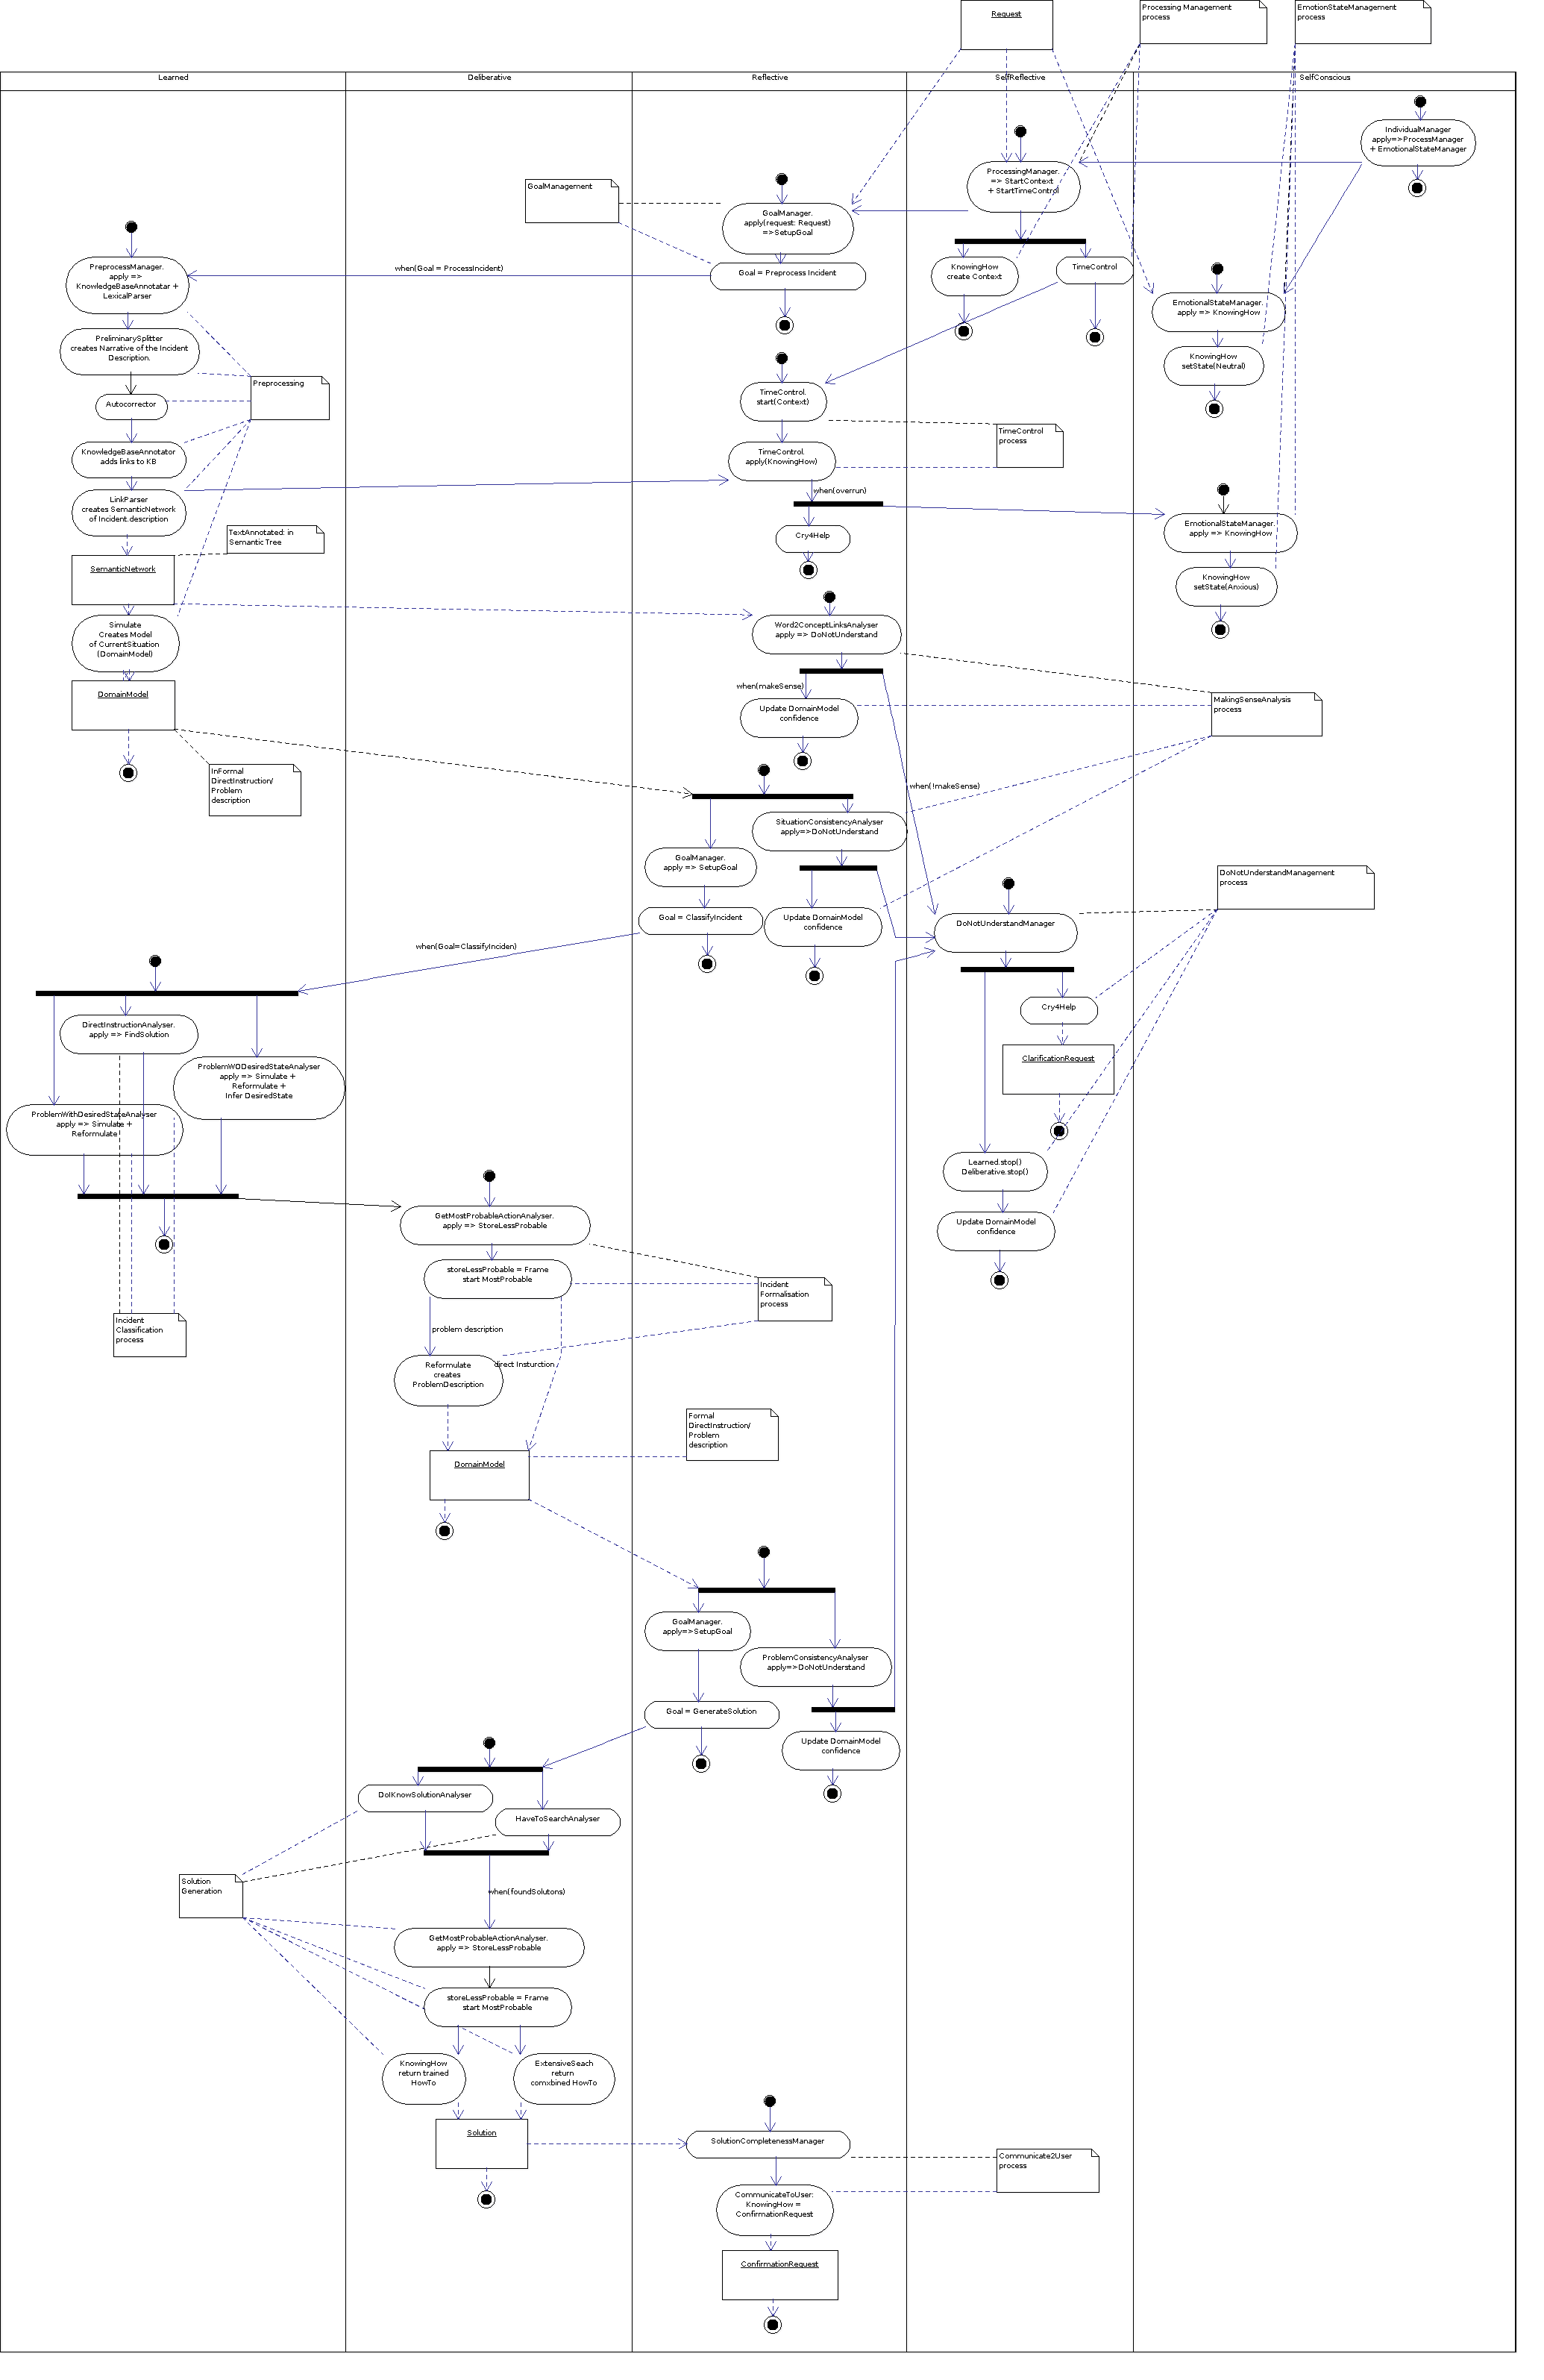
\includegraphics [scale=0.18] {LifecycleActivity}
  \caption{Диаграмма действий LifecycleActivity} 
  \label{img:LifecycleActivity}  
\end{figure}
\subsection{Технологии прототипа} \label{PrototypeTechnology}
Прототип был написан на языке Scala, с применением технологии Akka - параллельного исполнения на множестве ядер. В качестве базы используется Neo4j графовая база данных. 
\clearpage
\section{Апробация прототипа}
\subsection{Экспериментальные данные}
В качестве экспериментальных данных были взяты выгрузки данных из информационных систем из главы \ref{sect1_1}. 
Для обучения на базовом уровне в систему заложено две базовые концепции: 
\begin{itemize}
	\item Object - объект. Базовая концепция для всех объектов.
	\item Action - действие. Базовая концепция для всех действий.
\end{itemize} 
В таблице \ref{Test data description} представлен список основных тренировочных данных.

\begin{longtable}{|p{12cm}|p{5cm}|}
 \caption[Описание эксперементальных данных]{Описание эксперементальных данных}\label{Test data description} \\ 
 \hline
 
 \multicolumn{1}{|c|}{\textbf{Входное предложение}} & \multicolumn{1}{c|}{\textbf{Описание}}  \\ \hline 
\endfirsthead
\multicolumn{2}{c}%
{{\bfseries \tablename\ \thetable{} -- продолжение}} \\
\hline \multicolumn{1}{|c|}{\textbf{Входное предложение}} &
\multicolumn{1}{c|}{\textbf{Описание}}  \\ \hline 
\endhead

\hline \multicolumn{2}{|r|}{{Продолжение следует}} \\ \hline
\endfoot

\hline \hline
\endlastfoot
\hline
  Tense is kind of concept. & Обучающий запрос. Создает связь между концепцией Tense и Concept. \\
  
  \hline
  Please install Firefox.  & Запрос. Пользователь просит установить Firefox. Результатом должен быть найдено решение по установки Firefox. \\
  \hline
  Browser is an object.   & Обучающий запрос. Создает связь между концепцией Browser и object. \\
  \hline
  Firefox is a browser.   & Обучающий запрос. Создает связь между концепцией Firefox и browser.  \\
  \hline
  Install is an action.    & Обучающий запрос. Создает связь между концепцией Install и action. \\
  \hline
  User miss Internet Explorer 8.     & Запрос. Проблема с желаемым состоянием (DesiredState). \\
  \hline
  User needs document portal update.    & Запрос. Проблема с желаемым состоянием. \\
  \hline
  Add new alias Host name on host that alias is wanted to: hrportal.lalala.biz IP adress on host that alias is wanted to: 322.223.333.22 Wanted Alias:    webadviser.lalala.net    & Запрос. Сложная проблема.  \\ 
  \hline
  Outlook Web Access (CCC) - 403 - Forbidden: Access is denied & Запрос. Сложная проблема. \\ 
  \hline
  PP2C - Cisco IP communicator. Please see if you can fix the problem with the ip phone, it's stuck on configuring ip + sometimes Server error rejected: Security etc.     & Запрос. Сложная проблема. \\ 
   \hline
  \end{longtable}

Полный список информация об экспериментальных данных представлен в приложении \ref{AppendixE}
\clearpage
\subsection{Верификация}
Для доказания жизнеспособности решения произвожилась верификация в 2 этапа:
\begin{itemize}
	\item Этап 1. Разбор входящего запроса на естественном языке и вычленение концепции
	\item Этап 2. Обработка по разработанной архитектуре и реализации модели мышления  
\end{itemize}
Для Этапа 1 использовался отфильтрованная выгрузка инцидентов. Были выявлены уникальные инциденты - 1000. На данном этапе удалось добиться качества разбора на уровне 67\%. \\
Для Этапа 2 использовалась часть инцидентов, которая представлена в предыдущий главе. На них запускался программный комплекс и анализировались результаты. Удалось добиться 95\%. \\
\section{Выводы по главе}
В данной главе были представлены основные результаты работы:
\begin{itemize}
	\item Теоретико-множественный и теоретико-информационный анализ сложных систем в области поддержки информационной инфраструктуры
	\item Проблемно-ориентированная система управления, принятия решений и оптимизации технических объектов в области обслуживания IT
	\item Архитектура системы, ее реализация и испытания на модельных данных
\end{itemize}
Система показала свою жизнеспособность на модельных данных. 
%\newpage
%============================================================================================================================


\clearpage